%----------------------------------------------------------------------------
\chapter{Kísérlet}\label{sect:kiserlet}
%----------------------------------------------------------------------------

\texttt{+++ bevezeto a fejezethez +++}

%Szöveg.

%,,,,,,,,,,,,,,,,,,,,,,,,,,,,,,,,,,,,,,,,,,,,,,,,,,,,,,,,,,,,,,,,,,,,,,,,,,,,
\section{Módszerek összehasonlítása}\label{sect:modsz_osszehasonlitas}
%,,,,,,,,,,,,,,,,,,,,,,,,,,,,,,,,,,,,,,,,,,,,,,,,,,,,,,,,,,,,,,,,,,,,,,,,,,,,

\texttt{+++ miert BLOB-os keresest valasztottam Hough vagy Optical flow helyett? +++}

%,,,,,,,,,,,,,,,,,,,,,,,,,,,,,,,,,,,,,,,,,,,,,,,,,,,,,,,,,,,,,,,,,,,,,,,,,,,,
\section{Feldolgozási folyamat}\label{sect:feld_folyamat}
%,,,,,,,,,,,,,,,,,,,,,,,,,,,,,,,,,,,,,,,,,,,,,,,,,,,,,,,,,,,,,,,,,,,,,,,,,,,,

A blob alapú követést választva ki kellett dolgoznom a tekintetkövetés működéséhez szükséges képfeldolgozási illetve számítási folyamatot. Két feladatra kellett robusztus megoldást találnom: a pupilla követésére, valamint a pupilla-pozíció képernyő-pozícióba történő leképezésére.

%............................................................................
\subsection{Pupillakövetés}\label{sect:pupillakov}
%............................................................................

A pupillakövetés megbízható működéséhez meg kellett találnom az elemi képfeldolgozási műveletek megfelelő sorrendjét és paraméterezését. A pontos folyamat kialakítása nagyrészt intuíciók alapján, a részmegoldások folyamatos tesztelésével történt.

Az előfeldolgozási műveleteket az OpenCV készen kínálja, azonban a függvények száma és paraméterezési lehetőségei miatt rengeteg alternatíva jöhetett szóba. A szakasz további részében a kiválasztott képfeldolgozási műveleteket szeretném dokumentálni, a folyamat egészének tekintetében lényegtelen részletek mellőzésével. A felhasznált függvények pontos paraméterezése megtalálható az \sectref{parameterezes} függelékben.

\bigskip

A szemrégió képét közvetítő webkamera a gyári orientációjához képest fejjel lefelé került felfüggesztésre. A látványosabb megjelenítés érdekében ezért \emph{első lépésként} \textbf{megtükröztem} a képet a vízszintes középtengely mentén a \texttt{cv::flip} függvény használatával. Jegyezzük meg azonban, hogy ez a lépés csak azért szükséges, hogy a felhasználó számára könnyebben emészthető, ,,álló'' képet tudjunk megjeleníteni az alkalmazás felületén. A kép tükrözött voltát a feldolgozás során végig figyelembe véve ez a lépés akár el is hagyható.

A pupillakövetés szempontjából a színinformációnak nincs jelentősége, ezért a \emph{második lépés} a kép \textbf{szürkeárnyalatossá konvertálása} a \texttt{cv::cvtColor} metódus használatával.

A \emph{harmadik lépésben} \textbf{hisztogram-kiegyenlítést} végeztem a képen az OpenCV \texttt{cv::equalizeHist} függvénye használatával. A kiegyenlítés eredményeképp a kép minden megvilágítási körülmény között kellően kontrasztos lesz, megkönnyítve ezzel a pupilla detektálását.

TODO: hisztogram+kuszob

A szürkeárnyalatos képet ezek után a \emph{negyedik lépésben} \textbf{küszöbözni} kellett, ehhez a \texttt{cv::threshold} függvény használatára volt szükség. A pontos küszöbérték beállítása általában nehéz feladat, minden megvilágításra működő univerzális érték megtalálása pedig sokszor nem is lehetséges. A \sectref{infracam_mod} szakaszban részletezett infra-fényforrás megvalósításával azonban abba a szerencsés helyzetbe kerültem, hogy a külső megvilágítás hatását gyakorlatilag sikerült teljesen kiküszöbölni: a tesztelés során végül meghatározott ideális küszöbérték a verőfényes napsütéstől kezdve a vaksötét szobáig minden esetben megfelelően binarizálja a szürkeárnyalatos képet.

\bigskip

A fenti négy lépés elég a kamerakép előfeldolgozásához, az \emph{ötödik lépéstől} kezdve a tényleges felismerés megvalósítása következhet. Az előző, \sectref{modsz_osszehasonlitas} szakaszban kifejtettem, hogy a feldolgozás sebességét döntően befolyásolja a pixelszinten végzett feldolgozási lépések komplexitása és száma. A előfeldolgozás végén a kép még meglehetősen nagy zajjal terhelt: látható a pupilla viszonylag nagy, ovális foltja, azonban például a szempillák foltja zavaró hatásként jelentkezik.

Sebesség szempontjából azonban sokkal jobban járunk, ha nem is próbáljuk az előfeldolgozási lépések után hátramaradó zajt pixelszintű eljárásokkal kiszűrni (pl. bináris morfológia). Ehelyett az előfeldolgozott képre rögtön ráereszthetünk egy hierarchikus \textbf{kontúrkeresési eljárást} a \texttt{cv::findContours} függvény meghívásával. A további lépések során elegendő a hierarchia legfelső szintjét használnunk: mivel a megtalálni kívánt pupilla konvex, a blobok belsejében található lyukak elhelyezkedése nem szolgál többletinformációval.

\emph{Hatodik lépésben} meg is szabadulhatunk a \textbf{túl kis méretű objektumoktól}, mivel ezek nagy valószínűséggel csak mint zaj vannak jelen a képen. Egy kontúrpontjaival megadott objektum területét a \texttt{cv::contourArea} függvény segítségével határozhatjuk meg, ez alapján már kiszűrhetők a ,,túl kicsi'' objektumok.

A kisméretű zajok eltávolítása után jó eséllyel csak néhány, nagyobb területű blobunk marad, köztük a megtalálni kívánt pupilla. A fennmaradó blobok között jó szűrési feltételként adja magát a blobok \textbf{körkörösségének} vizsgálata. A \emph{hetedik lépésben} ezért a \sectref{blob_analizis} szakaszban ismertetett módon kiszámolom a foltok körkörösségi faktorát, majd ezek közül a legerősebbet kiválasztva nagyon jó százalékban sikerül a pupilla azonosítása.

Nincs más hátra, mint a \emph{nyolcadik lépésben} \textbf{ellipszist illeszteni} a pupilla kontúrjára, ehhez használható a \texttt{cv::fitEllipse} függvény. A pupillát a ráillesztett ellipszis paramétereivel lehet jellemezni: középpontjával, kis- és nagytengelyének hosszával, valamint nagytengelyének irányszögével.

\bigskip

A pupillakövetésnél gondolni kell azokra az esetekre is, amikor a követés fizikailag nem megvalósítható. Csukott szemnél a követés nyilvánvalóan lehetetlen, de az pislogási reflex okozta anomáliákat jó lenne kiszűrni. A detektálás közben felismerhető, ha egyáltalán nincs értékes pupilla-jelölt a blobok között. Abban az esetben, ha a fent vázolt algoritmus nem találja a pupillát, \textbf{öt egymást követő sikertelen felismerésig} még megtartja az utoljára detektált pupillapozíciót. Ezzel a módszerrel a pislogás okozta rövid kiesések szinte teljesen kiküszöbölhetők, és a valóban csukott szem detektálása is csak néhány századmásodperces késleltetést szenved.

%............................................................................
\subsection{Kalibráció, leképezés}\label{sect:kalibracio}
%............................................................................

\texttt{+++ kalibrálás + kepernyo-koordinataba kepzes +++}

%............................................................................
\section{Validáció}\label{sect:validacio}
%............................................................................

asdf

%,,,,,,,,,,,,,,,,,,,,,,,,,,,,,,,,,,,,,,,,,,,,,,,,,,,,,,,,,,,,,,,,,,,,,,,,,,,,
\section{Demonstráció}\label{sect:kiserletek}
%,,,,,,,,,,,,,,,,,,,,,,,,,,,,,,,,,,,,,,,,,,,,,,,,,,,,,,,,,,,,,,,,,,,,,,,,,,,,

\texttt{+++ leiras hogy miert ezekkel probaltam ki +++}

%............................................................................
\subsection{Pszichológiai bemutató}\label{sect:pszicho}
%............................................................................

A rendszer működését úgy demonstráltam, hogy végrehajtottam Alfred L. Yarbus orosz pszichológus 1967-es tanulmánya egy részletét. A kísérletben a kutatók azt bizonyították be, hogy a tesztalanyoknak előzetesen különböző kérdéseket feltéve, a kérdések jelentősen befolyásolták egy kép részleteinek vizsgálatát ahhoz képest, ha csak ,,szabadon'' nézegették azt. A teszteredményeket összefoglaló kép -- mint az egyik első a témával foglalkozó eredmény -- jól ismert a tekintetkövetéssel foglalkozók körében, ez látható a \figref{yarbus} ábrán.

\begin{figure}[!ht]
\centering
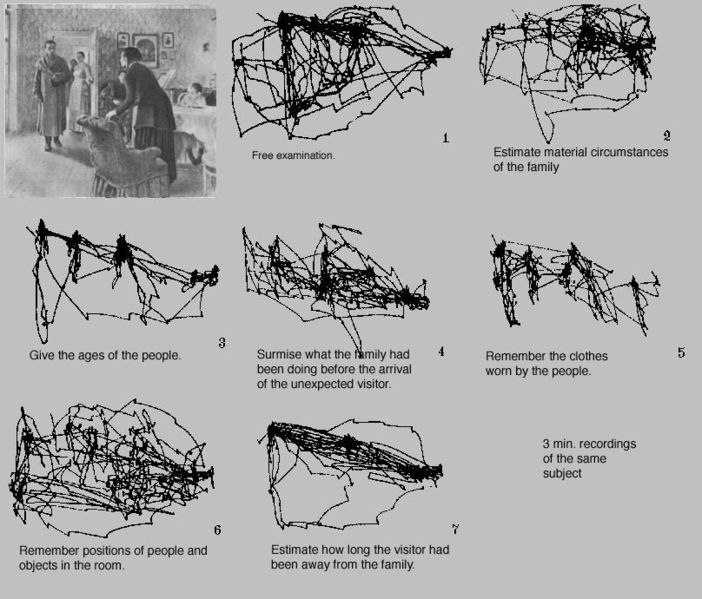
\includegraphics[width=140mm, keepaspectratio]{figures/yarbus.jpg}
\caption{Yarbus '67-es kísérletének eredménye}
\label{fig:yarbus}
\end{figure}

Látható, hogy a kísérlet végrehajtásához szükség volt a tekintet követésére. Ekkor még a kornak megfelelően nem álltak rendelkezésre kifinomult módszerek: az alanyokat egy meglehetősen kényelmetlen acélszerkezethez rögzítve vizsgálták. A bemutató alkalmazásomban arra kerestem a választ, hogy lehetséges-e hasonló méréseket elvégezni az általam fejlesztett rendszerrel.

\bigskip

Az általam tesztelt alanyoknak a következő kérdésekre kellett válaszolniuk a tesztkép (Repin: Váratlan utazó) rövid vizsgálata után. A vizsgálatot minden kérdésben 200 beérkezett érvényes mérési pontig folytattam, ez a felhasznált webkamera, illetve a feldolgozási sebesség mellett nagyjából kérdésenként 15--20 másodpercet vett igénybe.

\begin{enumerate}
 \item szabad nézelődés
 \item ,,Milyen anyagi körülmények között él a család?''
 \item ,,Adja meg az egyes szereplők életkorát!''
 \item ,,Mit csinálhattak a szereplők, mielőtt az utazó betoppant?''
 \item ,,Milyen ruhát viselnek a kép szereplői?''
 \item ,,Próbáljon megjegyezni minél több strukturális részletet (személyek, tárgyak pozíciója)!''
 \item ,,Mennyi ideig lehetett távol az utazó a családtól?''
\end{enumerate}

A kérdésekre nem volt jó, vagy rossz válasz, a kísérlet minden alanynál csak a feladatnak megfelelő figyelmi területek változását vizsgálja. A vizsgálatom eredménye a \figref{eredmeny} ábrán követhető.

\begin{figure}[!ht]
\centering
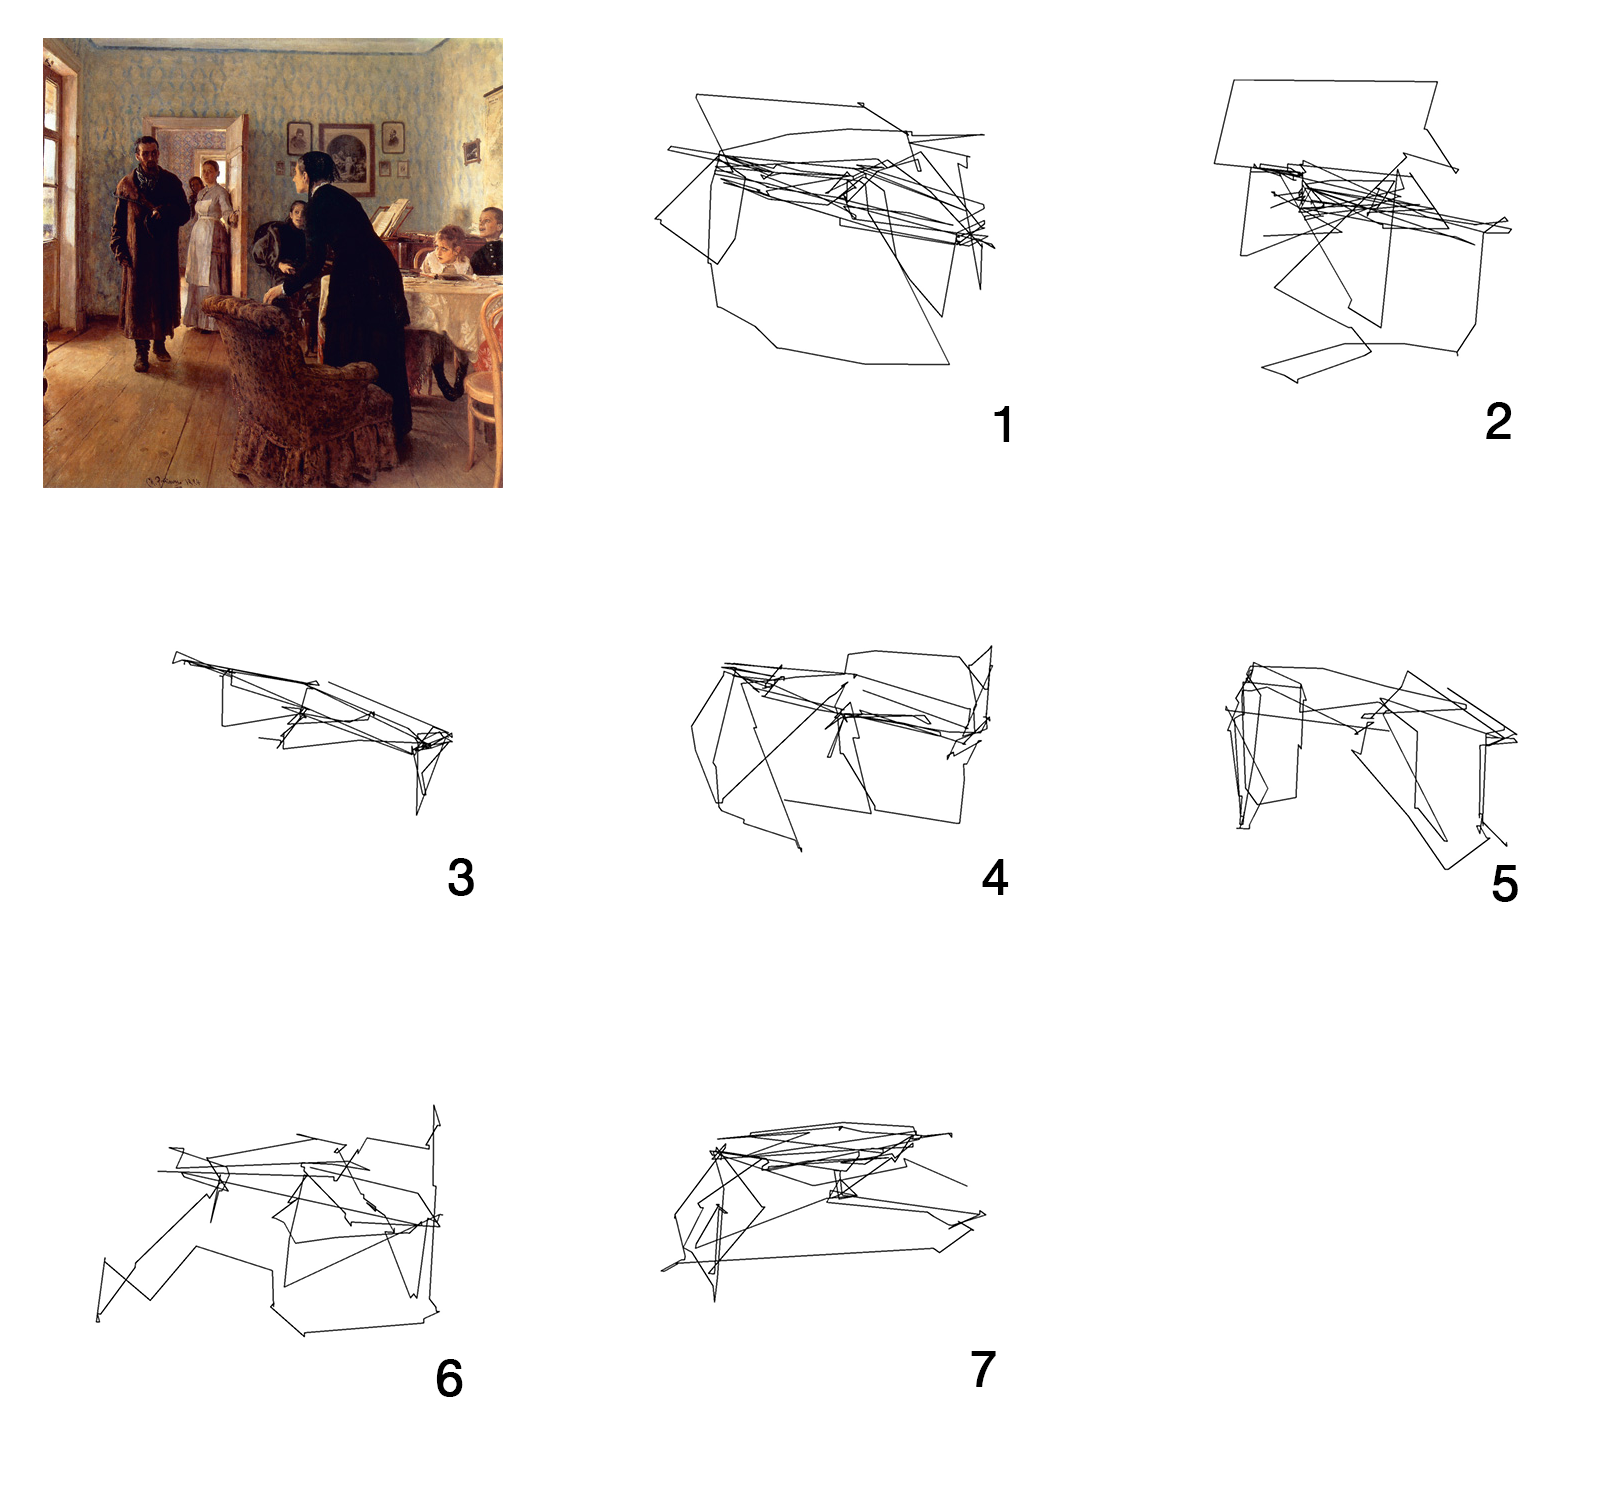
\includegraphics[width=140mm, keepaspectratio]{figures/yarbus_eredmeny.png}
\caption{Eredmények a saját rendszerrel}
\label{fig:eredmeny}
\end{figure}

Látható -- bár ez nem volt feltétel -- hogy a mérési eredmények ezen alany esetén meglehetősen jól fedik Yarbus tesztalanyának eredményeit. Az viszont mindenképpen kijelenthető, hogy szignifikáns különbség van az ábra első (szabad nézelődés), valamint többi része között. Nem célom a kísérlet pszichológiai eredményeit értékelni, az viszont bizonyos, hogy a rendszer hasonló kísérletek elvégzését támogatja.

%,,,,,,,,,,,,,,,,,,,,,,,,,,,,,,,,,,,,,,,,,,,,,,,,,,,,,,,,,,,,,,,,,,,,,,,,,,,,
\subsection{Webergonómiai bemutató}\label{sect:web}
%,,,,,,,,,,,,,,,,,,,,,,,,,,,,,,,,,,,,,,,,,,,,,,,,,,,,,,,,,,,,,,,,,,,,,,,,,,,,

Ahogyan dolgozatom első fejezetében már említettem, a tekintet követése a webergonómia területén is fontos kísérletek elvégzésére ad lehetőséget. A rendszer ilyen irányú képességeit demonstrálandó, elkészítettem az pszichológiai kísérlet adatait hőtérképen (heat map) megjelenítő funkciót is, ennek eredménye egy tesztképre a \figref{heatmap} ábrán látható.

\begin{figure}[!ht]
\centering
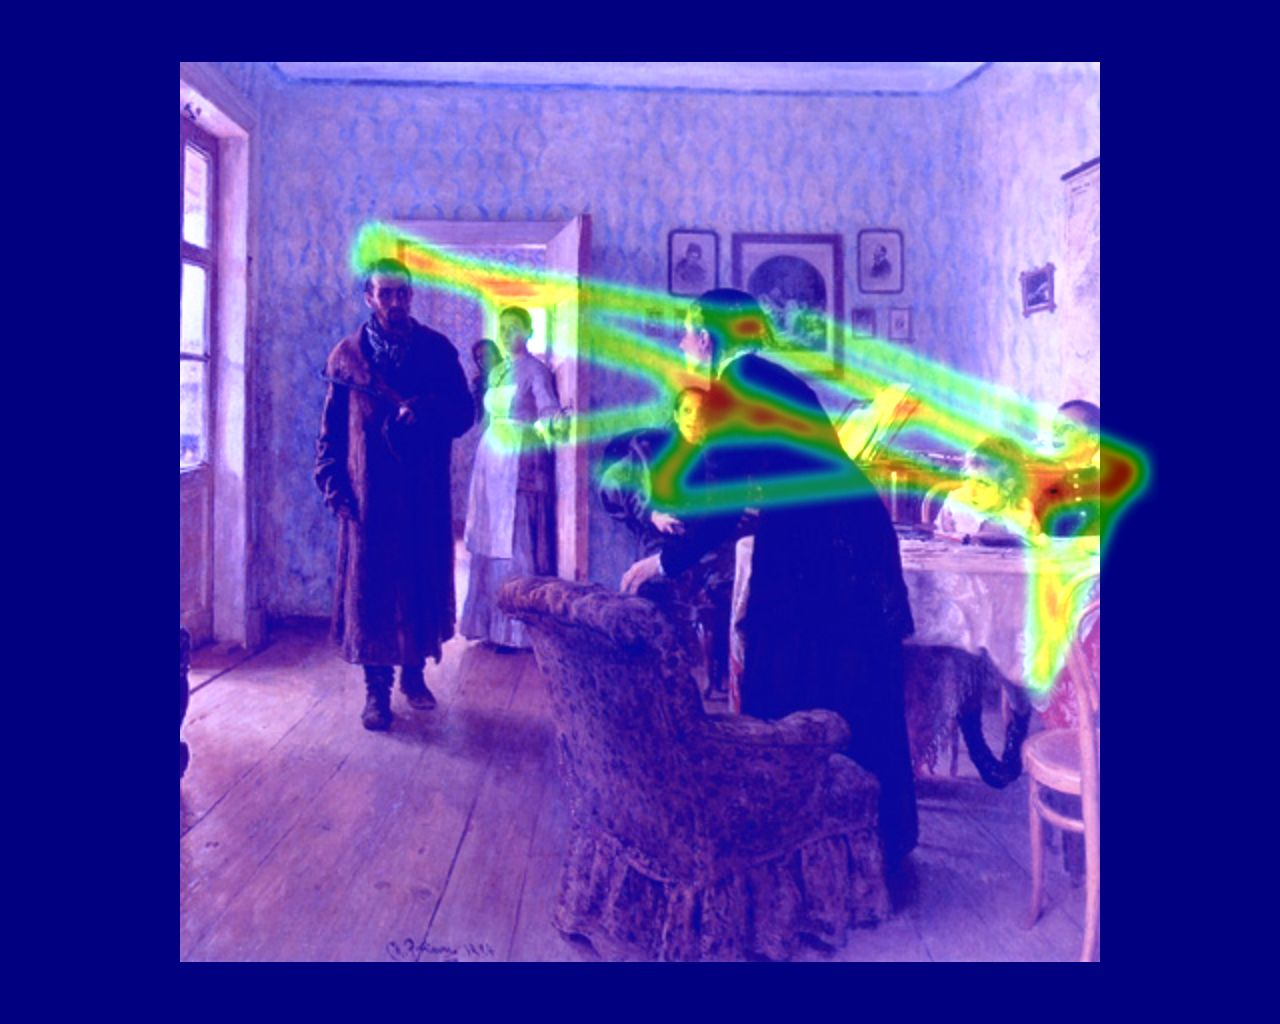
\includegraphics[width=100mm, keepaspectratio]{figures/heatmap.jpg}
\caption{Hőtérképes megjelenítés a pszichológiai teszt egy adathalmazára (,,Adja meg a szereplők életkorát!'')}
\label{fig:heatmap}
\end{figure}

Minden vizsgálatban célszerű a lehető leginkább informatív megjelenítést választani a rendelkezésre álló adathalmaz alapján. A képen egyre pirosabb színnel jelöltem a kép frekventáltan vizsgált területeit, például egy webergonómiai vizsgálatban az adatok effajta vizualizációja lehet a legcélszerűbb.

\bigskip

\texttt{+++ meg 1-2 bekezdes +++}

%,,,,,,,,,,,,,,,,,,,,,,,,,,,,,,,,,,,,,,,,,,,,,,,,,,,,,,,,,,,,,,,,,,,,,,,,,,,,
\section{Összefoglalás}\label{sect:kiserlet_osszefoglalas}
%,,,,,,,,,,,,,,,,,,,,,,,,,,,,,,,,,,,,,,,,,,,,,,,,,,,,,,,,,,,,,,,,,,,,,,,,,,,,

\texttt{+++ osszefoglalas a kiserletekrol +++}